\subsection*{Introducción}

Utilizando el método de simulación de Montecarlo y luego la transformación por autovectores estudiada en clase, es posible simular una variable aleatoria Gaussiana bidimensional correlacionada.

Se llevaron a cabo dos simulaciones con los siguientes parámetros.

\begin{center}
Caso 1: $\mu_{1} = 1$	 $\mu_{2} = 2$	 $\sigma_{1} = 0.5$	 $\sigma_{2} = 0.5$	 $\rho = 0.6$\label{eq:Parametros 1}

Caso 2: $\mu_{1} = 1$	 $\mu_{2} = 2$	 $\sigma_{1} = 0.5$	 $\sigma_{2} = 1$	 $\rho = 0.9$\label{eq:Parametros 2}

\end{center}

En primer lugar, se generó una muestra de puntos correspondientes a una Gaussiana bidimensional no correlacionada. Mediante el método de Montecarlo se generó una V.A. de distribución de Rayleigh y una V.A. uniforme, con ellas se obtuvo la Gaussiana bivariable. Luego, conociendo la matriz de covarianza requerida, se planteó la transformación lineal pertinente que llevo a una muestra correlacionada.
\\

\subsection*{Implementación}


El código en Matlab empleado en esta sección se reduce a archivo principal o main:
\begin{figure}[H]
	\centering
	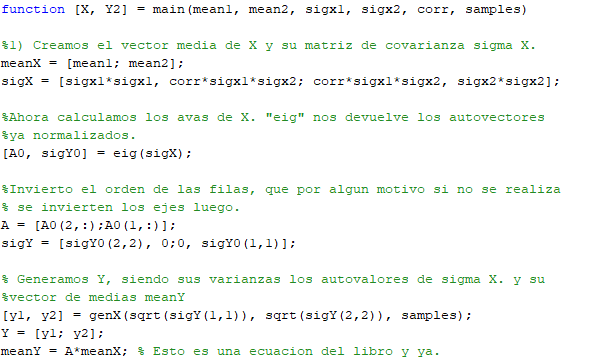
\includegraphics[width=0.6\linewidth]{./ImagenesEjercicio2/mainP1.PNG}
	\\
	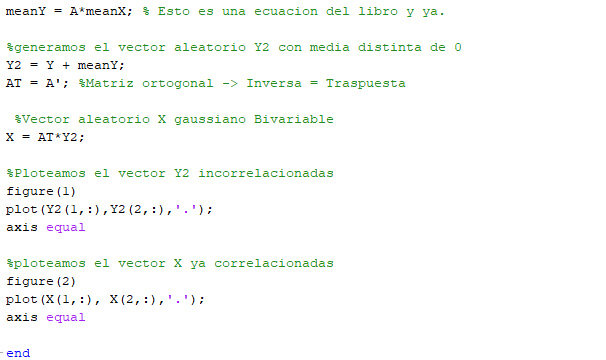
\includegraphics[width=0.6\linewidth]{./ImagenesEjercicio2/mainP2.PNG}
	\caption{Programa principal.}
	\label{fig:main}
\end{figure}

Donde las funciones utilizadas se definen a continuación:
La función genX genera las gaussianas incorrelacionas:
\begin{figure}[H]
	\centering
	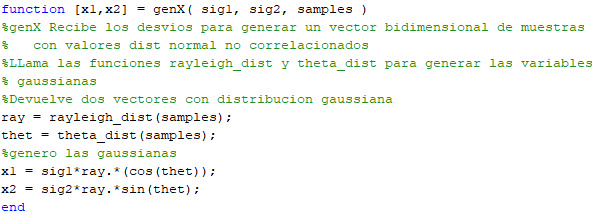
\includegraphics[width=0.6\linewidth]{./ImagenesEjercicio2/genX.PNG}
	\caption{Función genX.}
	\label{fig:genX}
\end{figure}

La función rayleigh dist que genera la simulación de una V.A. con distribución de Rayleigh:
\begin{figure}[H]
	\centering
	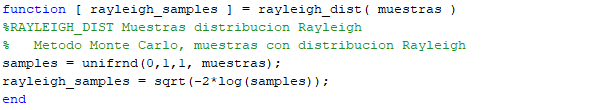
\includegraphics[width=0.6\linewidth]{./ImagenesEjercicio2/ray.PNG}
	\caption{Función rayleigh dist.}
	\label{fig:ray}
\end{figure}

La función theta dist que genera valores de un ángulo theta como V.A. de distribución uniforme:
\begin{figure}[H]
	\centering
	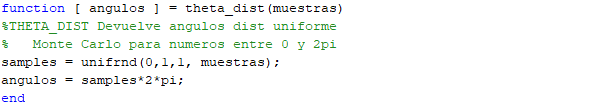
\includegraphics[width=0.6\linewidth]{./ImagenesEjercicio2/theta.PNG}
	\caption{Función theta dist.}
	\label{fig:theta}
\end{figure}

\subsection*{Resultados}

Se consideró a las V.A. con subindice 1 que se grafiquen en el eje X y con subíndice 2 en el eje Y. Las nubes de puntos que representan los vectores aleatorios se realizaron con 10000 muestras generadas por la distribución uniforme y la de rayleigh.

Para el caso 1 en la simulación se obtuvo la nube de puntos de una gaussiana bivariable no correlacionadas como en la siguiente figura:

\begin{figure}[H]
	\centering
	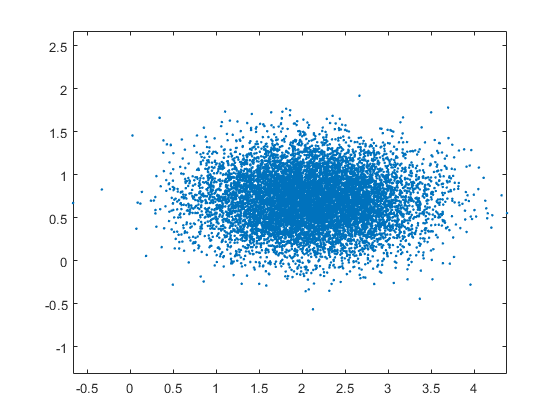
\includegraphics[width=0.5\linewidth]{./ImagenesEjercicio2/GaussianaBivariableSinCorr1.PNG}
	\caption{Caso 1, sin correlación.}
	\label{fig:G1SC}
\end{figure}

Luego, al aplicar la transformación, se obtiene la forma correlacionada de ambas gaussianas:

\begin{figure}[H]
	\centering
	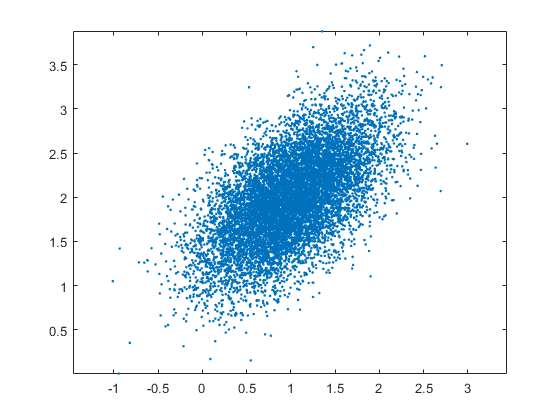
\includegraphics[width=0.4\linewidth]{./ImagenesEjercicio2/GaussianaBivariableCorr1.PNG}
	\caption{Caso 1, con correlación ($\rho$=0.6).}
	\label{fig:G1CC}
\end{figure}

También, se puede observar como quedaron ambas V.A. con distribución Gaussiana:

\begin{figure}[H]
	\centering
	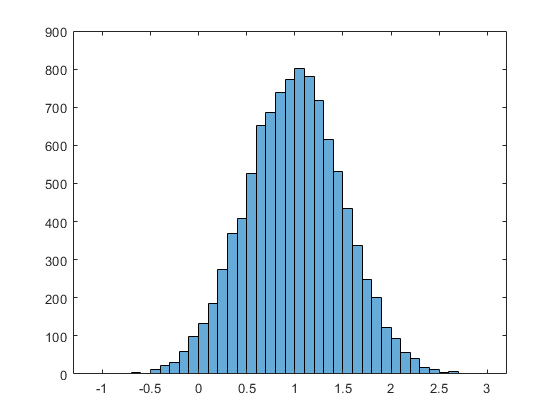
\includegraphics[width=0.5\linewidth]{./ImagenesEjercicio2/X1a.PNG}
	\caption{Variable X1 con $\mu_1$ = 1 y $\sigma_1$ = 0.5.}
	\label{fig:X1a}
\end{figure}
\begin{figure}[H]
	\centering
	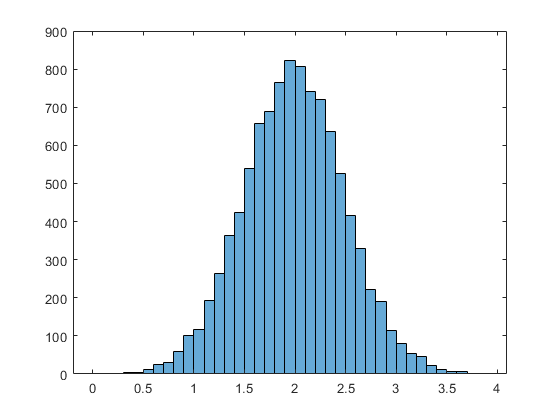
\includegraphics[width=0.5\linewidth]{./ImagenesEjercicio2/X2a.PNG}
	\caption{Variable X2 con $\mu_2$ = 2 y $\sigma_2$ = 0.5.}
	\label{fig:X2a}
\end{figure}

De igual manera para el caso 2, primero se obtuvieron las gaussianas no correlacionadas:

\begin{figure}[H]
	\centering
	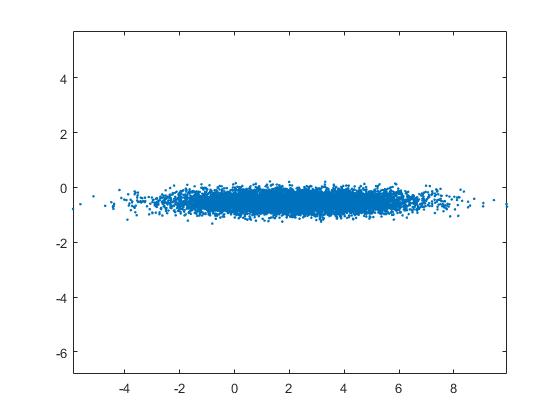
\includegraphics[width=0.5\linewidth]{./ImagenesEjercicio2/GaussianaBivariableSinCorr2.PNG}
	\caption{Caso 2, sin correlación.}
	\label{fig:C2SC}
\end{figure}

Nuevamente, aplicamos la transformación:

\begin{figure}[H]
	\centering
	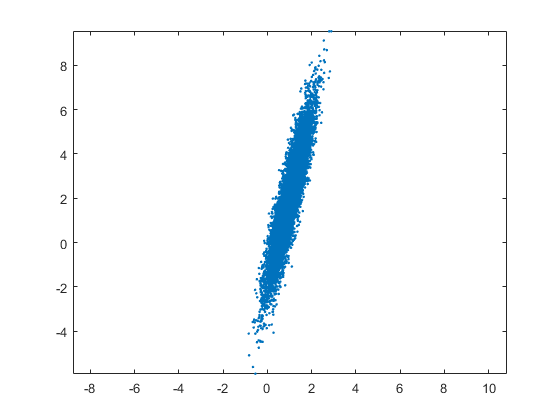
\includegraphics[width=0.5\linewidth]{./ImagenesEjercicio2/GaussianaBivariableCorr2.PNG}
	\caption{Caso 2, con correlación($\rho$=0.9).}
	\label{fig:C2CC}
\end{figure}

Finalmente, como observación las distribuciones de las V.A. gaussianas:

\begin{figure}[H]
	\centering
	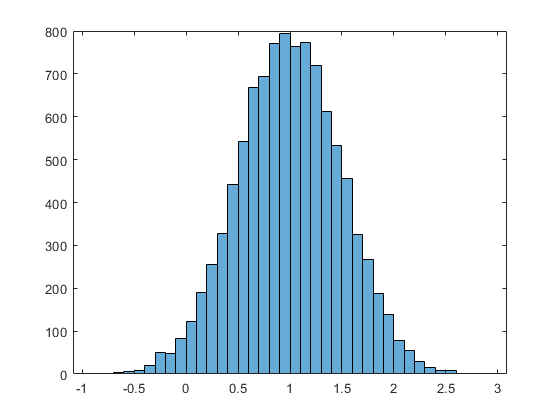
\includegraphics[width=0.5\linewidth]{./ImagenesEjercicio2/X1b.PNG}
	\caption{Variable X1 con $\mu_1$ = 1 y $\sigma_1$ = 0.5.}
	\label{fig:X1b}
\end{figure}
\begin{figure}[H]
	\centering
	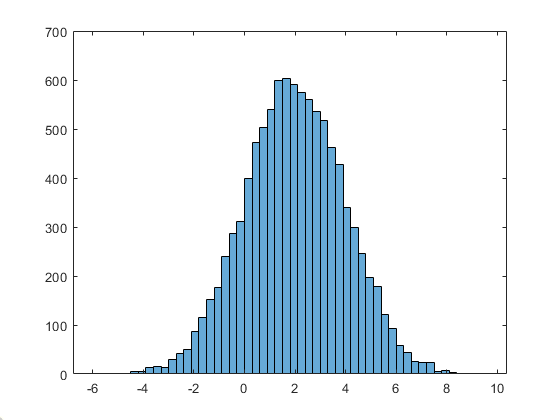
\includegraphics[width=0.5\linewidth]{./ImagenesEjercicio2/X2b.PNG}
	\caption{Variable X2 con $\mu_2$ = 2 y $\sigma_2$ = 2.}
	\label{fig:X2b}
\end{figure}

\subsection*{Análisis de resultados}

Se realizó de manera exitosa la simulación y obtención de una distribución gaussiana bimensional. Ambas simulaciones muestran los resultados esperados. En primer lugar, ambas nubes de puntos se pueden encontrar centradas en los puntos correspondientes a la media de cada eje según lo pedido.
Además se observa una orientación en la nube de los puntos que manifiesta la correlación entre las variables, nula en las Figuras (\ref{fig:G1SC}) y (\ref{fig:C2SC}), mientras que se presenta un claro cambio cuando se aplica la transformación que rota la nube de correlación de ambas variables, con $\rho=0.6$ en la Figura (\ref{fig:G1CC}) y $\rho= 0.9$ en la Figura (\ref{fig:C2CC}).
Por otra parte, ambas tienen valores de $\rho$ positivo y se observa que las pendientes de las nubes son positivas. En la segunda simulación, caso 2, la pendiente es mas precipitada, debido a que el factor de correlación es mayor como era de esperar.
Otra observación a destacar es que la diferencia en ancho de las muestras se atribuye a que en el caso 2 existe un mayor desvió en la V.A. graficada en el eje y, por lo cual la elipse se ve más ``alargada''.

Otra observación a destacar es que la diferencia en ancho de las muestras se atribuye a que en el caso 2 existe un mayor desvio en la V.A. graficada en el eje y, por lo cual la elipse se ve más "alargada" y esta tiende a una recta cuanto más se acerca $\rho$ a 1 o a -1.
